% !TEX root = ../../../main.tex

\begin{figure}[htb!]
    \centering
    \begin{subfigure}{0.18\textwidth}
        \caption*{Mode of agitation}
    \end{subfigure}
    \begin{subfigure}{0.18\textwidth}
        \caption*{\protect\raggedright Experimental crack network}
    \end{subfigure}
    \begin{subfigure}{0.19\textwidth}
        \caption*{$\Gc^*$}
        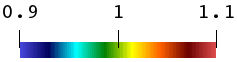
\includegraphics[width=\textwidth]{colorbar/rainbow_horizontal.png}
    \end{subfigure}
    \begin{subfigure}{0.19\textwidth}
        \caption*{$\pi_c^*$}
        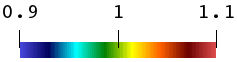
\includegraphics[width=\textwidth]{colorbar/rainbow_horizontal.png}
    \end{subfigure}
    \begin{subfigure}{0.19\textwidth}
        \caption*{$d$}
        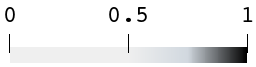
\includegraphics[width=\textwidth]{colorbar/grayscale_horizontal.png}
    \end{subfigure}

    \begin{subfigure}{0.18\textwidth}
        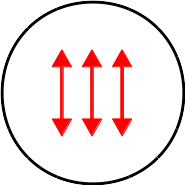
\includegraphics[width=\textwidth]{past/figures/brick_schematic.png}
    \end{subfigure}
    \begin{subfigure}{0.18\textwidth}
        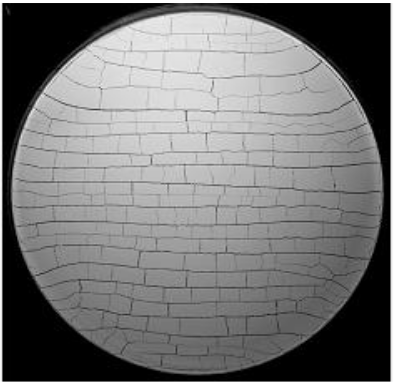
\includegraphics[width=\textwidth]{past/figures/paste_brick.png}
    \end{subfigure}
    \begin{subfigure}{0.19\textwidth}
        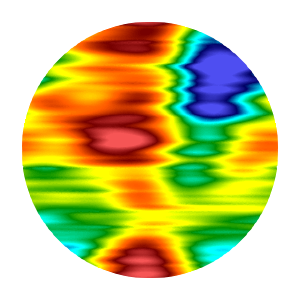
\includegraphics[width=\textwidth]{past/figures/Gc_brick.png}
    \end{subfigure}
    \begin{subfigure}{0.19\textwidth}
        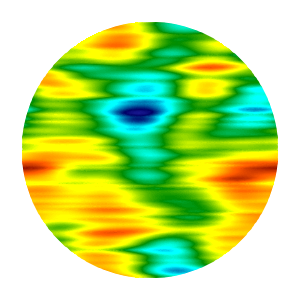
\includegraphics[width=\textwidth]{past/figures/psic_brick.png}
    \end{subfigure}
    \begin{subfigure}{0.19\textwidth}
        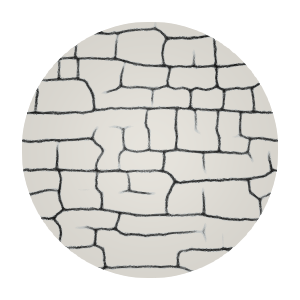
\includegraphics[width=\textwidth]{past/figures/d_brick.png}
    \end{subfigure}

    \begin{subfigure}{0.18\textwidth}
        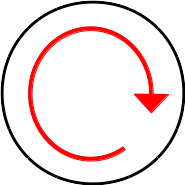
\includegraphics[width=\textwidth]{past/figures/radial_schematic.png}
    \end{subfigure}
    \begin{subfigure}{0.18\textwidth}
        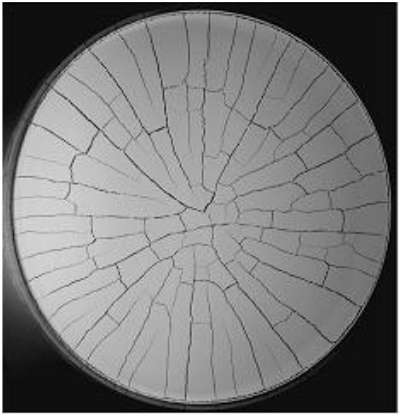
\includegraphics[width=\textwidth]{past/figures/paste_radial.png}
    \end{subfigure}
    \begin{subfigure}{0.19\textwidth}
        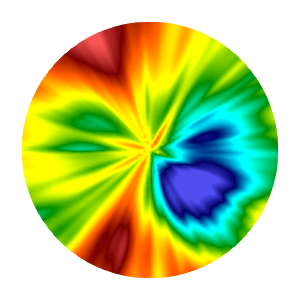
\includegraphics[width=\textwidth]{past/figures/Gc_radial.png}
    \end{subfigure}
    \begin{subfigure}{0.19\textwidth}
        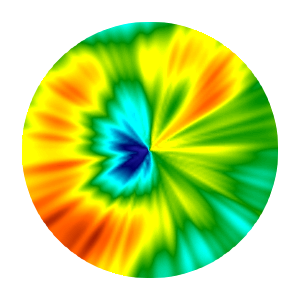
\includegraphics[width=\textwidth]{past/figures/psic_radial.png}
    \end{subfigure}
    \begin{subfigure}{0.19\textwidth}
        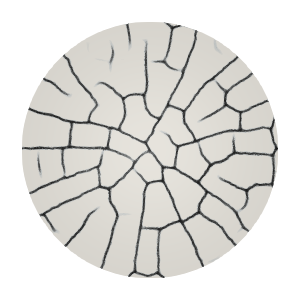
\includegraphics[width=\textwidth]{past/figures/d_radial.png}
    \end{subfigure}

    \begin{subfigure}{0.18\textwidth}
        
\includegraphics[width=\textwidth]{past/figures/ring_schematic.png}
    \end{subfigure}
    \begin{subfigure}{0.18\textwidth}
        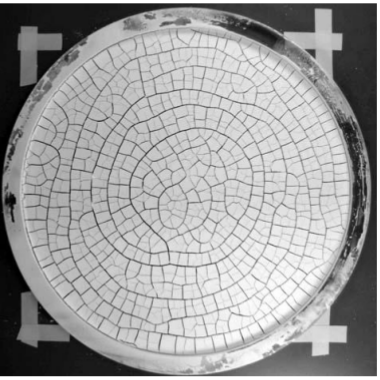
\includegraphics[width=\textwidth]{past/figures/paste_ring.png}
    \end{subfigure}
    \begin{subfigure}{0.19\textwidth}
        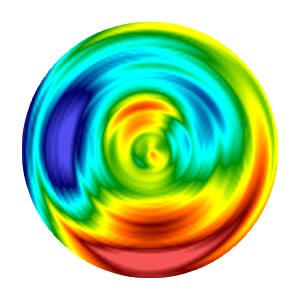
\includegraphics[width=\textwidth]{past/figures/Gc_ring.png}
    \end{subfigure}
    \begin{subfigure}{0.19\textwidth}
        
\includegraphics[width=\textwidth]{past/figures/psic_ring.png}
    \end{subfigure}
    \begin{subfigure}{0.19\textwidth}
        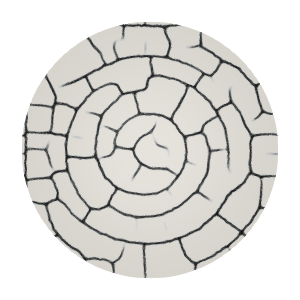
\includegraphics[width=\textwidth]{past/figures/d_ring.png}
    \end{subfigure}
\end{figure}
